\documentclass[a4paper,12pt]{report}

\usepackage{alltt, fancyvrb, url}
\usepackage{graphicx}
\usepackage[utf8]{inputenc}
\usepackage{float}
\usepackage{hyperref}
\usepackage{adjustbox}
\usepackage{siunitx}
\usepackage{tabularx}
\sisetup{group-separator={\text{\space}}}

% Questo commentalo se vuoi scrivere in inglese.
\usepackage[italian]{babel}

\usepackage[italian]{cleveref}

\title{Relazione per\\``Basi di dati''}

\author{Nicolò Guerra \and
Filippo Casadei}

\begin{document}

\maketitle

\tableofcontents

\chapter{Analisi dei requisiti}

Si vuole realizzare un database per la gestione di sistemi ospedalieri. Il sistema dovrà immagazzinare dati relativi a diverse ASL,
agli ospedali ad esse associate, pazienti, medici. Dovrà registrare inoltre referti relativi a visite, interventi e appuntamenti.

\section{Intervista}
Una prima descrizione delle richieste è la seguente:
\paragraph{}
Si vuole tenere traccia dei referti prodotti nei vari ospedali delle varie ASL della regione. Un referto può essere prodotto da un
intervento o da una visita/esame. Un referto è prodotto da un medico in un ospedale, ed è riferito ad un paziente. Dei pazienti si
vuole memorizzare nome, cognome, codice fiscale, data di nascita, numero di telefono, ASL di appartenenza e referti associati.
Di un impiegato si vuole memorizzare nome, cognome, codice fiscale e ruolo. Di un medico si vuole inoltre tenere traccia dello
storico degli interventi.
Un referto viene prodotto in una specifica data e nel caso sia di un intervento, si vuole sapere la procedura, l'esito, la durata e i medici
coinvolti. Nel caso sia di una visita invece si vuole avere una breve descrizione di quest'ultima e l'eventuale terapia prescritta.
Si vogliono memorizzare inoltre i seguenti dati per gli ospedali: nome, indirizzo, ASL di appartenenza, posti disponibili e persone
che lavorano in una struttura, e se questo dispone di un pronto soccorso.
Un ospedale si compone inoltre di più unità operative, ognuna caratterizzata da un nome, un dirigente, e dal personale che vi lavora.
Ogni ospedale ha delle attrezzature, identificate da un codice di inventario e di cui si vuole memorizzare il nome e la data dell'ultima
manutenzione.
Si vogliono infine memorizzare degli appuntamenti, che possono essere ad esempio prenotazioni per interventi e coinvolgono uno o più
pazienti e uno o più medici in una certa sala dell'ospedale ad una precisa data e ora. Un medico o un paziente non possono avere più
appuntamenti nello stesso momento. Una sala non può essere occupata da 2 appuntamenti contemporaneamente.
\section{Concetti principali da modellare}
\begin{itemize}
  \item ASL: Azienda sanitaria locale, gestisce la sanità di una singola zona di competenza, solitamente provinciale
  \item Ospedale: Struttura in cui avvengono visite e interventi dei pazienti
  \item Referto: Documento prodotto da un medico come resoconto di una visita o un intervento
  \item Paziente: Persona sottoposta a trattamenti ospedalieri
  \item Medico: Persona che lavora in un ospedale (o più di uno) e effettua trattamenti
  \item Impiegato: Persona che lavora in un ospedale ma non effettua trattamenti e non può firmare referti
  \item Unità operativa (U.O.): Reparto dell'ospedale specializzato in determinati tipi di trattamenti
  \item Attrezzatura: Macchinario utilizzato per particolari interventi e/o visite
  \item Appuntamento: Programmazione di visita o intervento
  \item Visita: Consulenza con un medico riguardante lo stato di salute del paziente
  \item Intervento: Operazione ad un paziente da parte di uno o più medici
  \item Sala: Stanza in cui avvengono visite e interventi
\end{itemize}
\section{Riscrittura dell'intervista corretta}
Di un referto si vuole memorizzare la data di emissione, il paziente, i medici coinvolti e il tipo di referto, oltre ad una breve descrizione.
Se è stato prodotto per un intervento si memorizzano anche procedura, esito e durata, se invece è per una visita la terapia prescritta.

Di una persona si vogliono memorizzare nome, cognome, codice fiscale, numero di telefono.
Di un paziente inoltre si vogliono memorizzare data di nascita, ASL di appartenenza e i referti associati.
Di un impiegato si vuole memorizzare il ruolo all'interno della struttura.
Di un medico si vuole memorizzare lo storico degli interventi.

Di un ospedale si vogliono memorizzare nome, indirizzo, ASL di appartenenza, posti disponibili (inteso come capienza totale in numero di pazienti),
persone che vi lavorano e il loro numero. Si vuole inoltre sapere se l'ospedale è munito di pronto soccorso.

Di una unità operativa si vogliono memorizzare il nome, l'ospedale a cui appartiene, il dirigente, il personale che vi lavora, la capienza e i posti liberi.

Di ogni attrezzatura si vogliono memorizzare il codice di inventario, l'ospedale di cui fanno parte, il nome e la data dell'ultima manutenzione.

Di ogni appuntamento si vuole memorizzare la data e l'ora, la durata stimata, il tipo, la sala, i pazienti e i medici coinvolti. 
Un paziente e/o un medico non possono avere più appuntamenti nello stesso lasso di tempo, inoltre una sala non può essere occupata da più 
appuntamenti allo stesso tempo.
\section{Principali azioni richieste}
\begin{itemize}
  \item Aggiungere un nuovo ospedale
  \item Aggiungere una nuova unità operativa
  \item Rimuovere un'unità operativa da un ospedale
  \item Aggiungere un nuovo paziente
  \item Aggiungere un nuovo impiegato/medico
  \item Fissare un appuntamento
  \item Cancellare un appuntamento
  \item Cambiare la data e/o il luogo di un appuntamento
  \item Aggiungere un nuovo referto
  \item Ricercare i referti per medico o per paziente
  \item Aggiungere nuova attrezzatura
  \item Rimuovere attrezzatura
  \item Aggiornare la data di manutenzione di un'attrezzatura
  \item Ricercare ospedali con determinate unità operative
  \item Ricerca di ospedali appartenenti ad un'ASL specifica
  \item Aggiungere una sala ad un ospedale
  \item Rimuovere una sala da un ospedale
  \item Ricercare ospedali con posti liberi in una determinata unità operativa
  \item Aggiungere pazienti in cura presso un ospedale
  \item Rimuovere un paziente in cura presso un ospedale
\end{itemize}

\chapter{Progettazione concettuale}
\begin{figure}[H]
	\centering{}
	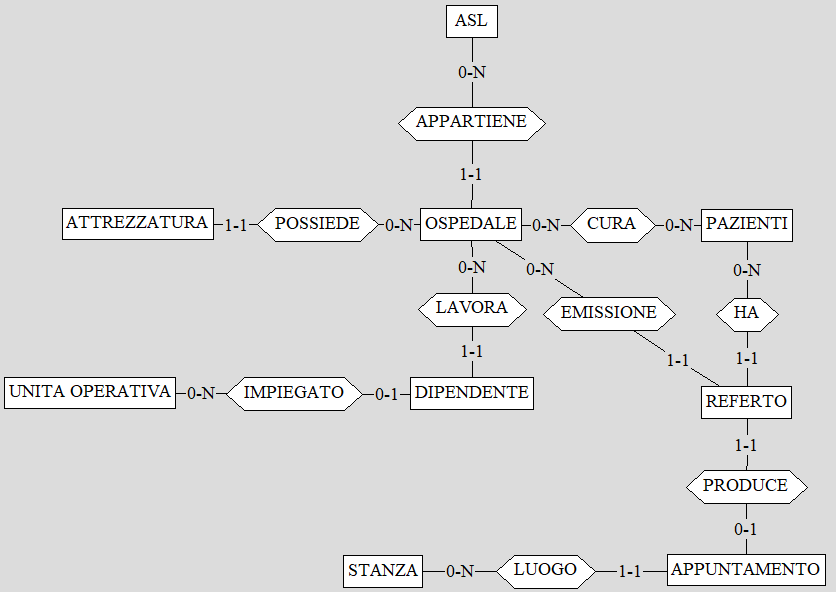
\includegraphics[width=\textwidth]{img/scheletro.png}
	\caption{Schema scheletro del problema.}
	\label{img:scheletro}
\end{figure}
Dopo l'esame del dominio del problema risultano alcune considerazioni da fare, che implicano diversi raffinamenti possibili:

Va considerata la presenza di diverse categorie di lavoratori all'interno di un ospedale e solo alcuni di questi devono essere in grado di rilasciare
referti ai pazienti. Per questi motivi si è deciso di dividere l'entità dipendenti dello schema scheletro in amministrativi e personale sanitario, che assieme a pazienti
risultano essere sottocategorie dell'entità persona, identificabili mediante codice fiscale.

Inoltre unicamente gli amministrativi sono collegati direttamente all'ospedale, mentre il personale sanitario si relaziona ad un'unità operativa, quest'ultima associata 
ad un ospedale.

Gli appuntamenti vengono modellati come entità perché devono essere identificati da data, ora e luogo in cui avvengono, attributi propri dell'appuntamento 
stesso. Non risultano però modellabili alcuni requisiti. Essendo gli appuntamenti protratti nel tempo non si può modellare nello schema E-R il vincolo di 
non poter avere 2 appuntamenti sovrapposti. Diversamente da come descritto sopra un appuntamento non è direttamente connesso ad un referto, ma esprime
unicamente il concetto di incontro tra un pazienti e medici.

Anche visite e interventi sono estensioni della generica entità referto, ne rappresentano infatti il tipo, e i dati specifici per l'uno o per l'altro caso. Inoltre per
poter ricostruire lo storico degli interventi di un medico ogni referto è anche associato al medico che lo ha prodotto.

È stata anche aggiunta la relazione di registrazione di un paziente presso una determinata ASL.

Lo schema E/R definitivo risulta quindi essere il seguente:
\begin{figure}[p]
  \begin{adjustbox}{addcode={\begin{minipage}{\width}}{\caption{%
    Schema E/R del problema.
    }\end{minipage}},rotate=270,center}
    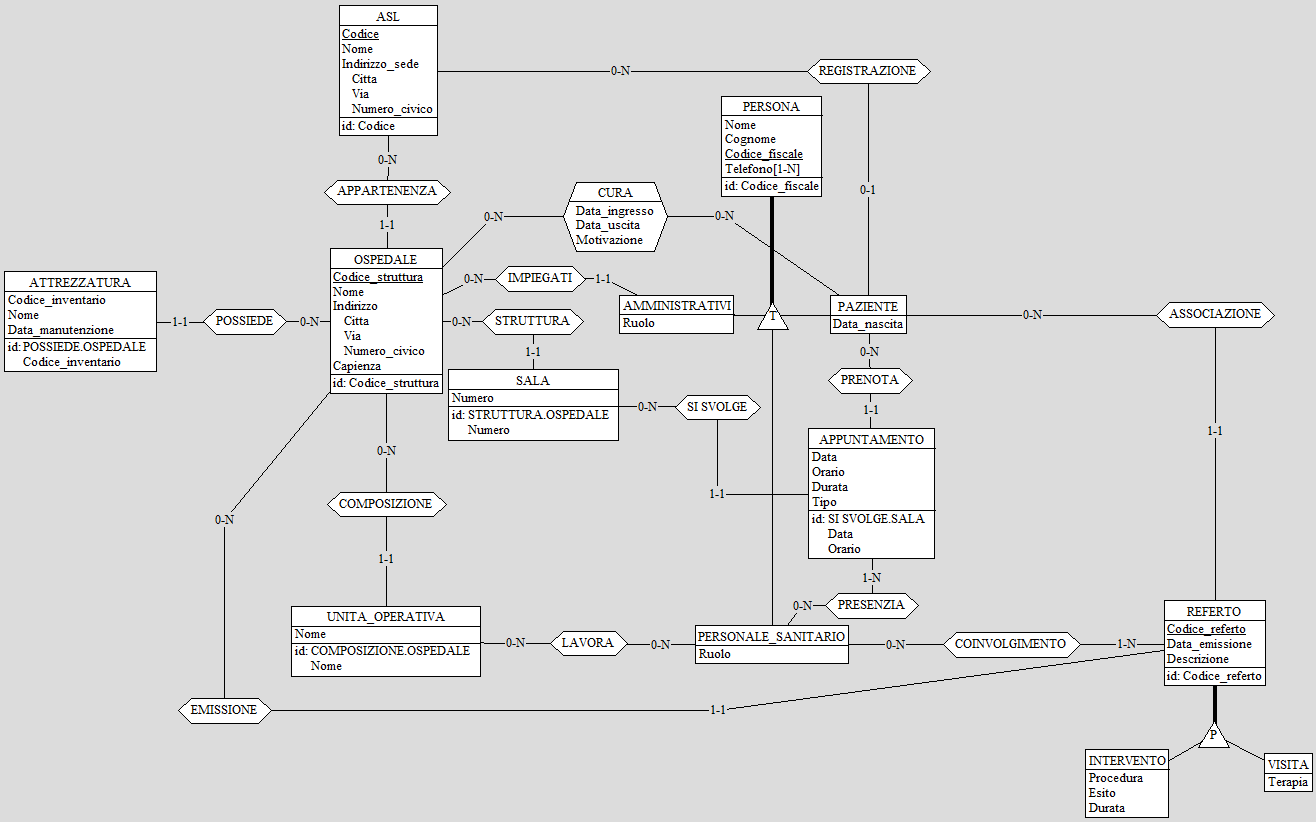
\includegraphics[height=0.93\textwidth]{img/er_final.png}
    \label{img:er}
  \end{adjustbox}
\end{figure}

\chapter{Progettazione logica}
\section{Stima del volume dei dati}
Si stimano nella tabella seguente il volume dei dati previsto nel database:
\subsection{Entità}
\begin{center}
  \begin{tabular}{ c | S[table-format=8.0, table-space-text-pre=(, table-space-text-post=)] }
    Nome & Quantità \\
    \hline
    Amministrativi & 40000 \\
    Appuntamento & 12000000 \\
    ASL & 100 \\
    Attrezzatura & 15000 \\
    Intervento & 200000 \\
    Ospedale & 1000 \\
    Paziente & 50000000 \\
    Persona & 51000000 \\
    Personale sanitario & 500000 \\
    Sala & 30000 \\
    Unità operativa & 10000\\
    Visita & 7000000 \\
  \end{tabular}
\end{center}
 
Va considerato che essendo Personale sanitario, Amministrativi e Paziente gerarchie di persona il loro volume è 
sovrapposto (la copertura è totale ma non esclusiva). 
Anche Intervento e Visita sono gerarchie di Referto, ma essendo questa volta una copertura totale e disgiunta Referto
è stato omesso perché ricavabile come somma di queste 2.
I volumi di Intervento e Visita sono inoltre calcolati su un anno di operatività. Questo perché sono dati che crescono molto rapidamente 
e si rende necessario un sistema di archiviazione a lungo termine per evitare di sovraccaricare il sistema e causare inefficienze.
Anche gli appuntamenti soffrono dello stesso problema, per cui vengono eliminati una volta effettuati.

\subsection{Relazioni}
\begin{center}
  \begin{tabular}{ c | S[table-format=8.0, table-space-text-pre=(, table-space-text-post=)] }
    Nome & Quantità \\
    \hline
    Appartenenza & 1000 \\
    Associazione & 7200000 \\
    Coinvolgimento & 8800000 \\
    Composizione & 10000 \\
    Cura & 6000000 \\
    Emissione & 7200000 \\
    Impiegati & 40000 \\
    Lavora & 700000 \\
    Possiede & 15000 \\
    Prenota & 12000000 \\
    Presenzia & 15000000 \\
    Registrazione & 45000000 \\
    Si svolge & 12000000 \\
    Struttura & 30000 \\
  \end{tabular}
\end{center}

Si consideri che come nella sezione precedente anche qui alcuni dati sono stati stimati su un anno di operatività. 
Cura è una relazione che cambia rapidamente nel tempo e per evitare il sovraccarico del sistema va archiviata a intervalli regolari.

\subsection{Principali operazioni e loro frequenza}
Segue ora una tabella in cui vengono riportate le principali operazioni da effettuare sul database e la loro frequenza stimata.
\begin{center}
  \begin{tabular}{ p{269pt} | l }
    Operazione & Frequenza \\
    \hline
    \hline
    Aggiungere un nuovo ospedale & 3 all'anno \\
    Aggiungere una nuova unità operativa & 25 all'anno \\
    Rimuovere un'unità operativa da un ospedale & 10 all'anno \\
    Aggiungere un nuovo paziente & 1000 al giorno \\
    Aggiungere un nuovo impiegato/medico & 2000 al mese \\
    Fissare un appuntamento & 30000 al giorno \\
    Cancellare un appuntamento & 3000 al giorno \\
    Cambiare la data e/o il luogo di un appuntamento & 2000 al giorno \\
    Aggiungere un nuovo referto & 10000 al giorno \\
    Ricercare i referti per medico o per paziente & 7000 al giorno \\
    Aggiungere nuova attrezzatura & 40 all'anno \\
    Rimuovere attrezzatura & 30 all'anno \\
    Aggiornare la data di manutenzione di un'attrezzatura & 22500 all'anno \\
    Ricercare ospedali con determinate unità operative & 750 al giorno \\
    Ricerca di ospedali appartenenti ad un'ASL specifica & 15000 al giorno \\
    Aggiungere una sala ad un ospedale & 10 all'anno \\
    Rimuovere una sala da un ospedale & 5 all'anno \\
    Ricercare ospedali con posti liberi in una determinata unità operativa & 200 al giorno \\
    Aggiungere pazienti in cura presso un ospedale & 12500 al giorno \\
    Rimuovere un paziente in cura presso un ospedale & 12500 al giorno \\
  \end{tabular}
\end{center}
\subsection{Dettaglio delle operazioni e tabelle degli accessi}
Sono ora descritte le operazioni nel dettaglio con la stima del loro costo e le tabelle degli accessi. A questo fine gli 
accessi in scrittura vengono considerati di costo doppio rispetto a quelli in lettura.

Per operazioni particolarmente complesse vengono inoltre riportati gli schemi di navigazione.

\subsubsection*{1 - Aggiungere un nuovo ospedale}
Conoscendo già il codice dell'ASL a cui l'ospedale da aggiungere dovrà appartenere questa operazione richiede la scrittura dell'entità ospedale 
e della sua relazione con ASL (appartenenza).
\vspace{6pt}
\newline
\begin{tabularx}{\textwidth}{ 
  | >{\centering\arraybackslash}X 
  | >{\centering\arraybackslash}X 
  | >{\centering\arraybackslash}X 
  | >{\centering\arraybackslash}X |}
  \hline
  Soggetto & E/R & Accessi & R/W \\
  \hline
  \hline
  Ospedale & E & 1 & W \\ 
  \hline
  Appartenenza & R & 1 & W \\
  \hline
\end{tabularx}
\vspace{3pt}\newline
Costo operazione: 1W + 1W = 4 \newline Costo totale: 4 * 3 (all'anno) = 12 all'anno

\subsubsection*{2 - Aggiungere una nuova unità operativa}
Conoscendo già il codice dell'ospedale a cui l'unità operativa verrà aggiunta questa operazione richiede la scrittura dell'entità unità operativa 
e della sua relazione con ospedale (composizione).
\vspace{6pt}
\newline
\begin{tabularx}{\textwidth}{ 
  | >{\centering\arraybackslash}X 
  | >{\centering\arraybackslash}X 
  | >{\centering\arraybackslash}X 
  | >{\centering\arraybackslash}X |}
  \hline
  Soggetto & E/R & Accessi & R/W \\
  \hline
  \hline
  Unità operativa & E & 1 & W \\ 
  \hline
  Composizione & R & 1 & W \\
  \hline
\end{tabularx}
\vspace{3pt}\newline
Costo operazione: 1W + 1W = 4 \newline Costo totale: 4 * 25 (all'anno) = 100 all'anno

\subsubsection*{3 - Rimuovere un'unità operativa da un ospedale}
Rimuovere un unità operativa significa rimuovere anche la sua associazione con l'ospedale a cui apparteneva e l'associazione del personale sanitario 
attualmente assegnato a quell'unità, in media 40 per unità.
\vspace{6pt}
\newline
\begin{tabularx}{\textwidth}{ 
  | >{\centering\arraybackslash}X 
  | >{\centering\arraybackslash}X 
  | >{\centering\arraybackslash}X 
  | >{\centering\arraybackslash}X |}
  \hline
  Soggetto & E/R & Accessi & R/W \\
  \hline
  \hline
  Unità operativa & E & 1 & W \\ 
  \hline
  Composizione & R & 1 & W \\
  \hline
  Lavora & R & 40 & W \\
  \hline
\end{tabularx}
\vspace{3pt}\newline
Costo operazione: 1W + 1W + 40W = 84 \newline Costo totale: 84 * 10 (all'anno) = 840 all'anno

\subsubsection*{4 - Aggiungere un nuovo paziente}
Aggiungere un paziente richiede la scrittura di una tupla nell'entità \emph{Paziente}. Viene considerata anche la scrittura della relazione \emph{Registrazione}
nonostante non sia obbligatoria perché la quasi totalità dei pazienti è registrata presso un'ASL.
\vspace{6pt}
\newline
\begin{tabularx}{\textwidth}{ 
  | >{\centering\arraybackslash}X 
  | >{\centering\arraybackslash}X 
  | >{\centering\arraybackslash}X 
  | >{\centering\arraybackslash}X |}
  \hline
  Soggetto & E/R & Accessi & R/W \\
  \hline
  \hline
  Paziente & E & 1 & W \\ 
  \hline
  Registrazione & R & 1 & W \\
  \hline
\end{tabularx}
\vspace{3pt}\newline
Costo operazione: 1W + 1W = 4 \newline Costo totale: 4 * 1000 (al giorno) = 4000 al giorno

\subsubsection*{5 - Aggiungere un nuovo impiegato/medico}
Aggiungere un medico, assumendo che le unità operative vengano assegnate in un secondo momento, richiede una nuova tupla nell'entità \emph{Personale sanitario}.
\vspace{6pt}
\newline
\begin{tabularx}{\textwidth}{ 
  | >{\centering\arraybackslash}X 
  | >{\centering\arraybackslash}X 
  | >{\centering\arraybackslash}X 
  | >{\centering\arraybackslash}X |}
  \hline
  Soggetto & E/R & Accessi & R/W \\
  \hline
  \hline
  Personale sanitario & E & 1 & W \\ 
  \hline
\end{tabularx}
\vspace{3pt}\newline
Costo operazione: 1W = 2 \newline Costo totale: 2 * 1200 (al mese) = 2400 al mese
\vspace{3pt}
\newline
Aggiungere un impiegato invece richiede la scrittura di una tupla in \emph{Personale amministrativo}, e della relazione \emph{Impiegati}.
\vspace{6pt}
\newline
\begin{tabularx}{\textwidth}{ 
  | >{\centering\arraybackslash}X 
  | >{\centering\arraybackslash}X 
  | >{\centering\arraybackslash}X 
  | >{\centering\arraybackslash}X |}
  \hline
  Soggetto & E/R & Accessi & R/W \\
  \hline
  \hline
  Amministrativi & E & 1 & W \\
  \hline
  Impiegati & R & 1 & W \\
  \hline
\end{tabularx}
\vspace{3pt}\newline
Costo operazione: 2W = 4 \newline Costo totale: 4 * 800 (al mese) = 3200 al mese

\subsubsection*{6 - Fissare un appuntamento}
Fissare un appuntamento richiede di verificare che il medico non sia occupato in un altro appuntamento e che la sala sia libera in un dato orario.
Per controllare che il medico non sia occupato è necessario leggere gli appuntamenti di un medico in una certa data, quindi un numero pari alla media
di appuntamenti giornalieri di un medico dalla relazione \emph{Presenzia}, dopodiche leggere dall'entità \emph{Appuntamento} quanti di questi hanno orario e durata
tali da sovrapporsi a quello che stiamo inserendo. Dobbiamo poi leggere gli appuntamenti che si svolgono in un giorno in una stanza e controllare anche qui se ci sono
sovrapposizioni.
% TODO: INSERIRE SCHEMA DI NAVIGAZIONE
\vspace{6pt}
\newline
\begin{tabularx}{\textwidth}{ 
  | >{\centering\arraybackslash}X 
  | >{\centering\arraybackslash}X 
  | >{\centering\arraybackslash}X 
  | >{\centering\arraybackslash}X |}
  \hline
  Soggetto & E/R & Accessi & R/W \\
  \hline
  Presenzia & R & 4 & R \\
  \hline
  Si svolge & R & 8 & R \\
  \hline
  Appuntamento & E & 1 & W \\
  \hline
  Si svolge & R & 1 & W \\
  \hline
  Prenota & R & 1 & W \\
  \hline
  Presenzia & R & 1 & W \\
  \hline
\end{tabularx}
\vspace{3pt}\newline
Costo operazione: 4R + 8R + 1W + 1W + 1W + 1W = 20 \newline Costo totale: 20 * 30000 (al giorno) = 600000 al giorno

\subsubsection*{7 - Cancellare un appuntamento}
Cancellare un appuntamento richiede di eliminare la relativa tupla dall'entità appuntamento, e le 3 relazioni che la caratterizzano. In condizioni
normali una visita è presieduta da un solo medico, quindi si considera questo caso ai fini del calcolo dei costi.
\vspace{6pt}
\newline
\begin{tabularx}{\textwidth}{ 
  | >{\centering\arraybackslash}X 
  | >{\centering\arraybackslash}X 
  | >{\centering\arraybackslash}X 
  | >{\centering\arraybackslash}X |}
  \hline
  Soggetto & E/R & Accessi & R/W \\
  \hline
  Appuntamento & E & 1 & W \\
  \hline
  Prenota & R & 1 & W \\
  \hline
  Si svolge & R & 1 & W \\
  \hline
  Presenzia & R & 1 & W \\
  \hline
\end{tabularx}
\vspace{3pt}\newline
Costo operazione: 1W + 1W + 1W + 1W = 8 \newline Costo totale: 8 * 3000 (al giorno) = 24000 al giorno

\subsubsection*{8 - Cambiare la data o il luogo dell'appuntamento}
Cambiare data e ora di un appuntamento conoscendo la nuova data e ora e la nuova sala in cui si svolgerà richiede solamente di effettuare un aggiornamento
sull'entità \emph{Appuntamento} e una sulla relazione \emph{Si svolge}.
\vspace{6pt}
\newline
\begin{tabularx}{\textwidth}{ 
  | >{\centering\arraybackslash}X 
  | >{\centering\arraybackslash}X 
  | >{\centering\arraybackslash}X 
  | >{\centering\arraybackslash}X |}
  \hline
  Soggetto & E/R & Accessi & R/W \\
  \hline
  Appuntamento & E & 1 & W \\
  \hline
  Si svolge & R & 1 & W \\
  \hline
\end{tabularx}
\vspace{3pt}\newline
Costo operazione: 1W + 1W = 4 \newline Costo totale: 4 * 2000 (al giorno) = 8000 al giorno

\subsubsection*{9 - Aggiungere un nuovo referto}
\emph{Referto} è un'entità che ha come sotto entità nella gerarchia \emph{Intervento} e \emph{Visita}, essendo però una copertura totale ed esclusiva e non avendo le 
sotto entità altre relazioni, consideriamo solo \emph{Referto} nel calcolo dei costi per l'inserimento. La media delle associazioni \emph{Coinvolgimento} tra \emph{Personale sanitario}
e \emph{Referto} è ottenuta considerando che la maggioranza delle visite è tra un solo medico e il paziente, mentre quasi tutti gli interventi richiedono più personale.
% TODO: INSERIRE SCHEMA DI NAVIGAZIONE
\vspace{6pt}
\newline
\begin{tabularx}{\textwidth}{ 
  | >{\centering\arraybackslash}X 
  | >{\centering\arraybackslash}X 
  | >{\centering\arraybackslash}X 
  | >{\centering\arraybackslash}X |}
  \hline
  Soggetto & E/R & Accessi & R/W \\
  \hline
  Referto & E & 1 & W \\
  \hline
  Associazione & R & 1 & W \\
  \hline
  Emissione & R & 1 & W \\
  \hline
  Coinvolgimento & R & 2 & W \\
  \hline
\end{tabularx}
\vspace{3pt}\newline
Costo operazione: 1W + 1W + 1W + 2W = 10 \newline Costo totale: 10 * 10000 (al giorno) = 100000 al giorno

\subsubsection*{10 - Ricercare i referti per medico o per paziente}
Ricercare i referti per paziente assumendo di conoscere già il codice fiscale del paziente richiede di leggere tutte le tuple legate a quel paziente in \emph{Associazione},
e quindi tutti i referti associati. Si considerano 2 referti per ogni persona come media. Dato che è necessario sapere dove un referto è stato emesso e chi è coinvolto si
considerano anche le letture di queste relazioni.
% TODO: INSERIRE SCHEMA DI NAVIGAZIONE
\vspace{6pt}
\newline
\begin{tabularx}{\textwidth}{ 
  | >{\centering\arraybackslash}X 
  | >{\centering\arraybackslash}X 
  | >{\centering\arraybackslash}X 
  | >{\centering\arraybackslash}X |}
  \hline
  Soggetto & E/R & Accessi & R/W \\
  \hline
  Associazione & R & 2 & R \\
  \hline
  Referto & E & 2 & R \\
  \hline
  Emissione & R & 2 & R \\
  \hline
  Coinvolgimento & R & 2 & R \\
  \hline
\end{tabularx}
\vspace{3pt}\newline
Costo operazione: 2L + 2L + 2L + 2L = 8 \newline Costo totale: 8 * 6000 (al giorno) = 48000 al giorno
\vspace{3pt}
\newline
Ricercare i referti associati ad un medico richiede invece la lettura in coinvolgimento di tutte le associazioni \emph{Coinvolgimento} tra quel medico e un referto. 
Dopodiche si procede a ricostruire le relazioni di \emph{Referto} come sopra.
\vspace{6pt}
\newline
\begin{tabularx}{\textwidth}{ 
  | >{\centering\arraybackslash}X 
  | >{\centering\arraybackslash}X 
  | >{\centering\arraybackslash}X 
  | >{\centering\arraybackslash}X |}
  \hline
  Soggetto & E/R & Accessi & R/W \\
  \hline
  \hline
  Coinvolgimento & R & 18 & R \\
  \hline
  Referto & E & 18 & R \\
  \hline
  Associazione & R & 18 & R \\
  \hline
  Emissione & R & 18 & R \\
  \hline
\end{tabularx}
\vspace{3pt}\newline
Costo operazione: 18R + 18R + 18R + 18R = 72 \newline Costo totale: 72 * 1000 (al giorno) = 72000 al giorno

\subsubsection*{11 - Aggiungere nuova attrezzatura}
L'aggiunta di nuova attrezzatura richiede di aggiungere una tupla all'entità \emph{Attrezzatura}, e di registrare la sua associazione \emph{Possiede} con l'ospedale.
\vspace{6pt}
\newline
\begin{tabularx}{\textwidth}{ 
  | >{\centering\arraybackslash}X 
  | >{\centering\arraybackslash}X 
  | >{\centering\arraybackslash}X 
  | >{\centering\arraybackslash}X |}
  \hline
  Soggetto & E/R & Accessi & R/W \\
  \hline
  Attrezzatura & E & 1 & W \\
  \hline
  Possiede & R & 1 & W \\
  \hline
\end{tabularx}
\vspace{3pt}\newline
Costo operazione: 1W + 1W = 4 \newline Costo totale: 4 * 40 (all'anno) = 160 all'anno

\subsubsection*{12 - Rimuovere attrezzatura}
La rimozione dell'attrezzatura richiede di rimuovere una tupla dall'entità \emph{Attrezzatura}, e di eliminare la sua associazione \emph{Possiede} con l'ospedale.
\vspace{6pt}
\newline
\begin{tabularx}{\textwidth}{ 
  | >{\centering\arraybackslash}X 
  | >{\centering\arraybackslash}X 
  | >{\centering\arraybackslash}X 
  | >{\centering\arraybackslash}X |}
  \hline
  Soggetto & E/R & Accessi & R/W \\
  \hline
  Attrezzatura & E & 1 & W \\
  \hline
  Possiede & R & 1 & W \\
  \hline
\end{tabularx}
\vspace{3pt}\newline
Costo operazione: 1W + 1W = 4 \newline Costo totale: 4 * 30 (all'anno) = 120 all'anno

\subsubsection*{12 - Aggiornare la data di manutenzione di un’attrezzatura}
L'aggiornamento della data di ultima manutenzione dell'attrezzatura richiede di aggiornare una tupla nell'entità \emph{Attrezzatura}.
\vspace{6pt}
\newline
\begin{tabularx}{\textwidth}{ 
  | >{\centering\arraybackslash}X 
  | >{\centering\arraybackslash}X 
  | >{\centering\arraybackslash}X 
  | >{\centering\arraybackslash}X |}
  \hline
  Soggetto & E/R & Accessi & R/W \\
  \hline
  Attrezzatura & E & 1 & W \\
  \hline
\end{tabularx}
\vspace{3pt}\newline
Costo operazione: 1W = 2 \newline Costo totale: 2 * 22500 (all'anno) = 45000 all'anno

\subsubsection*{13 - Ricercare ospedali con determinate unità operative}
Ricercare ospedali con determinate unità operative richiede di leggere tutte le tuple di \emph{Composizione} con unità operativa corrispondente a quella richiesta, e da quelle
leggere le tuple dell'entità \emph{Ospedale} associate.
\vspace{6pt}
\newline
\begin{tabularx}{\textwidth}{ 
  | >{\centering\arraybackslash}X 
  | >{\centering\arraybackslash}X 
  | >{\centering\arraybackslash}X 
  | >{\centering\arraybackslash}X |}
  \hline
  Soggetto & E/R & Accessi & R/W \\
  \hline
  Composizione & R & 140 & R \\
  \hline
  Ospedale & E & 140 & R \\
  \hline
\end{tabularx}
\vspace{3pt}\newline
Costo operazione: 140R + 140R = 280 \newline Costo totale: 280 * 750 (al giorno) = 210000 al giorno

\subsubsection*{14 - Ricerca di ospedali appartenenti ad un’ASL specifica}
La ricerca di ospedali appartenenti ad una specifica ASL assumendo di conoscerne il codice richiede un numero di letture della relazione \emph{Appartenenza} pari
al numero medio di ospedali per ASL.
\vspace{6pt}
\newline
\begin{tabularx}{\textwidth}{ 
  | >{\centering\arraybackslash}X 
  | >{\centering\arraybackslash}X 
  | >{\centering\arraybackslash}X 
  | >{\centering\arraybackslash}X |}
  \hline
  Soggetto & E/R & Accessi & R/W \\
  \hline
  Appartenenza & R & 10 & R \\
  \hline
  Ospedale & E & 10 & R \\
  \hline
\end{tabularx}
\vspace{3pt}\newline
Costo operazione: 10R + 10R = 20 \newline Costo totale: 20 * 15000 (al giorno) = 300000 al giorno

\subsubsection*{15 - Aggiungere una sala ad un ospedale}
L'aggiunta di una sala ad un ospedale richiede l'aggiunta di una tupla all'entità \emph{Sala} e della sua associazione \emph{Struttura} con ospedale.
\vspace{6pt}
\newline
\begin{tabularx}{\textwidth}{ 
  | >{\centering\arraybackslash}X 
  | >{\centering\arraybackslash}X 
  | >{\centering\arraybackslash}X 
  | >{\centering\arraybackslash}X |}
  \hline
  Soggetto & E/R & Accessi & R/W \\
  \hline
  Sala & E & 1 & W \\
  \hline
  Struttura & R & 1 & W \\
  \hline
\end{tabularx}
\vspace{3pt}\newline
Costo operazione: 1W + 1W = 4 \newline Costo totale: 4 * 10 (all'anno) = 40 all'anno

\subsubsection*{16 - Rimuovere una sala da un ospedale}
La rimozione di una sala da un ospedale richiede la rimozione di una tupla dall'entità \emph{Sala} e della sua associazione \emph{Struttura} con ospedale.
Non viene considerata la rimozione degli appuntamenti associati a quella sala perché è opportuno non rimuoverla qualora ci siano degli appuntamenti fissati ma prima spostare
questi ultimi in altre sale.
\vspace{6pt}
\newline
\begin{tabularx}{\textwidth}{ 
  | >{\centering\arraybackslash}X 
  | >{\centering\arraybackslash}X 
  | >{\centering\arraybackslash}X 
  | >{\centering\arraybackslash}X |}
  \hline
  Soggetto & E/R & Accessi & R/W \\
  \hline
  Sala & E & 1 & W \\
  \hline
  Struttura & R & 1 & W \\
  \hline
\end{tabularx}
\vspace{3pt}\newline
Costo operazione: 1W + 1W = 4 \newline Costo totale: 4 * 5 (all'anno) = 20 all'anno

\subsubsection*{17 - Ricercare ospedali con posti liberi in una determinata unità operativa}
Inanzitutto è necessario ricercare le unità operative corrispondenti a quella richiesta e i cui posti occupati siano inferiori alla capienza.
Infine dall'unità bisogna risalire all'ospedale attraverso la relazione \emph{Composizione}. Di tutte le unità operative vengono considerate corrispondenti
a quella cercata 1 su 70, e di queste con posti liberi i \( \frac{3}{4} \).
% TODO: INSERIRE SCHEMA DI NAVIGAZIONE
\vspace{6pt}
\newline
\begin{tabularx}{\textwidth}{ 
  | >{\centering\arraybackslash}X 
  | >{\centering\arraybackslash}X 
  | >{\centering\arraybackslash}X 
  | >{\centering\arraybackslash}X |}
  \hline
  Soggetto & E/R & Accessi & R/W \\
  \hline
  Unità operative & E & 105 & R \\
  \hline
  Ospedale & E & 105 & R \\
  \hline
\end{tabularx}
\vspace{3pt}\newline
Costo operazione: 105R + 105R = 210 \newline Costo totale: 210 * 200 (al giorno) = 42000 al giorno

\subsubsection*{18 - Aggiungere pazienti in cura presso un ospedale}
Bisogna controllare che un paziente non sia già in cura presso una struttura, leggendo le tuple di cura associate a un paziente e controllare se ne esistono
senza l'attributo data di uscita. Diamo per scontato che si cerchi di aggiungere un paziente ad un unità operativa che non è piena. Per aggiungere un paziente 
in cura presso un ospedale è sufficiente aggiungere una tupla alla relazione \emph{Cura} e aggiornare i posti occupati nell'unità operativa.
% TODO: INSERIRE SCHEMA DI NAVIGAZIONE
\vspace{6pt}
\newline
\begin{tabularx}{\textwidth}{ 
  | >{\centering\arraybackslash}X 
  | >{\centering\arraybackslash}X 
  | >{\centering\arraybackslash}X 
  | >{\centering\arraybackslash}X |}
  \hline
  Soggetto & E/R & Accessi & R/W \\
  \hline
  Cura & R & 10 & R \\
  \hline
  Cura & R & 1 & W \\
  \hline
  Unità operativa & E & 1 & W \\
  \hline 
\end{tabularx}
\vspace{3pt}\newline
Costo operazione: 10R + 1W + 1W = 14 \newline Costo totale: 14 * 12500 (al giorno) = 175000 al giorno

\subsubsection*{19 - Rimuovere un paziente in cura}
Per rimuovere un paziente in cura presso un ospedale è sufficiente aggiornare la tupla nella relazione \emph{Cura} con la data di uscita del paziente e aggiornare 
i posti occupati nell'unità operativa.
% TODO: INSERIRE SCHEMA DI NAVIGAZIONE
\vspace{6pt}
\newline
\begin{tabularx}{\textwidth}{ 
  | >{\centering\arraybackslash}X 
  | >{\centering\arraybackslash}X 
  | >{\centering\arraybackslash}X 
  | >{\centering\arraybackslash}X |}
  \hline
  Soggetto & E/R & Accessi & R/W \\
  \hline
  Cura & R & 1 & W \\
  \hline
  Unità operativa & E & 1 & W \\
  \hline 
\end{tabularx}
\vspace{3pt}\newline
Costo operazione: 1W + 1W = 4 \newline Costo totale: 4 * 12500 (al giorno) = 50000 al giorno

\section{Raffinamento dello schema}
\subsection{Analisi delle ridondanze}
\subsubsection*{Capienza unità operative}
L'attributo \emph{Posti\textunderscore occupati} dell'entità \emph{Unità operativa} è ridondante, in quanto sarebbe deducibile dalla relazione \emph{Cura} contando le tuple corrispondenti
a quell'unità operativa che non contengono l'attributo \emph{Data\textunderscore uscita}.

Segue l'analisi del costo delle operazioni interessate:

\subsubsection*{17 - Ricercare ospedali con posti liberi in una determinata unità operativa}
\textbf{Con ridondanza:}
\vspace{6pt}
\newline
\begin{tabularx}{\textwidth}{ 
  | >{\centering\arraybackslash}X 
  | >{\centering\arraybackslash}X 
  | >{\centering\arraybackslash}X 
  | >{\centering\arraybackslash}X |}
  \hline
  Soggetto & E/R & Accessi & R/W \\
  \hline
  Unità operativa & E & 105 & R \\
  \hline
  Ospedale & E & 105 & R \\
  \hline
\end{tabularx}
\vspace{3pt}\newline
Costo operazione: 105R + 105R = 210 \newline Costo totale: 210 * 200 (al giorno) = 42000 al giorno
\vspace{6pt}
\newline
\textbf{Senza ridondanza:}
\vspace{6pt}
\newline
\begin{tabularx}{\textwidth}{ 
  | >{\centering\arraybackslash}X 
  | >{\centering\arraybackslash}X 
  | >{\centering\arraybackslash}X 
  | >{\centering\arraybackslash}X |}
  \hline
  Soggetto & E/R & Accessi & R/W \\
  \hline
  Unità operativa & E & 140 & R \\
  \hline
  Cura & R & 1400 & R \\
  \hline
  Composizione & R & 105 & R \\
  \hline
  Ospedale & E & 105 & R \\
  \hline
\end{tabularx}
\vspace{3pt}\newline
Costo operazione: 140R + 1400R + 105R + 105R = 1750 \newline Costo totale: 1750 * 200 (al giorno) = 350000 al giorno

\subsubsection*{18 - Aggiungere pazienti in cura presso un ospedale}
\textbf{Con ridondanza:}
\vspace{6pt}
\newline
\begin{tabularx}{\textwidth}{ 
  | >{\centering\arraybackslash}X 
  | >{\centering\arraybackslash}X 
  | >{\centering\arraybackslash}X 
  | >{\centering\arraybackslash}X |}
  \hline
  Soggetto & E/R & Accessi & R/W \\
  \hline
  Cura & R & 10 & R \\
  \hline
  Cura & R & 1 & W \\
  \hline
  Unità operativa & E & 1 & W \\
  \hline 
\end{tabularx}
\vspace{3pt}\newline
Costo operazione: 10R + 1W + 1W = 14 \newline Costo totale: 14 * 12500 (al giorno) = 175000 al giorno
\newline
\textbf{Senza ridondanza:}
\vspace{6pt}
\newline
\begin{tabularx}{\textwidth}{ 
  | >{\centering\arraybackslash}X 
  | >{\centering\arraybackslash}X 
  | >{\centering\arraybackslash}X 
  | >{\centering\arraybackslash}X |}
  \hline
  Soggetto & E/R & Accessi & R/W \\
  \hline
  Cura & R & 10 & R \\
  \hline
  Cura & R & 1 & W \\
  \hline 
\end{tabularx}
\vspace{3pt}\newline
Costo operazione: 10R + 1W = 12 \newline Costo totale: 12 * 12500 (al giorno) = 150000 al giorno

\subsubsection*{19 - Rimuovere un paziente in cura}
\textbf{Con ridondanza:}
\vspace{6pt}
\newline
\begin{tabularx}{\textwidth}{ 
  | >{\centering\arraybackslash}X 
  | >{\centering\arraybackslash}X 
  | >{\centering\arraybackslash}X 
  | >{\centering\arraybackslash}X |}
  \hline
  Soggetto & E/R & Accessi & R/W \\
  \hline
  Cura & R & 1 & W \\
  \hline
  Unità operativa & E & 1 & W \\
  \hline 
\end{tabularx}
\vspace{3pt}\newline
Costo operazione: 1W + 1W = 4 \newline Costo totale: 4 * 12500 (al giorno) = 50000 al giorno
\newline
\textbf{Senza ridondanza:}
\vspace{6pt}
\newline
\begin{tabularx}{\textwidth}{ 
  | >{\centering\arraybackslash}X 
  | >{\centering\arraybackslash}X 
  | >{\centering\arraybackslash}X 
  | >{\centering\arraybackslash}X |}
  \hline
  Soggetto & E/R & Accessi & R/W \\
  \hline
  Cura & R & 1 & W \\
  \hline 
\end{tabularx}
\vspace{3pt}\newline
Costo operazione: 1W = 2 \newline Costo totale: 2 * 12500 (al giorno) = 25000 al giorno
\vspace{3pt}
\newline
Totale con ridondanza: 42000 + 175000 + 150000 = 367000. 
\newline
Totale senza ridondanza: 350000 + 150000 + 25000 = 525000.
\vspace{3pt}
\newline
Risulta chiaro che la ridondanza riduce significativamente il carico sul sistema, quindi verrà mantenuto.

\subsection{Eliminazione delle gerarchie}
\subsubsection*{Referto}
La gerarchia di \emph{Referto} è stata eliminata con un collasso verso l'alto. Questo perché accedendo al referto si vuole accedere anche alle relative
informazioni contenute nelle entità figlie \emph{Intervento} e \emph{Visita}, e queste ultime non hanno ulteriori relazioni. Si è quindi deciso di accorpare gli attributi 
di entrambe le entità figlie nell'entità padre e aggiungere un attributo di tipo per semplificare lo schema.
\begin{figure}[H]
	\centering{}
	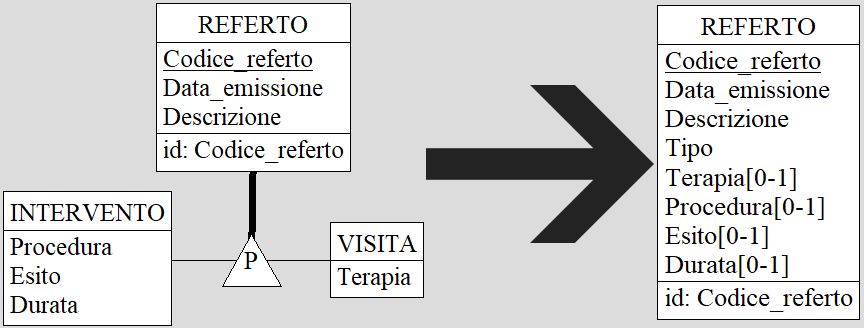
\includegraphics[width=\textwidth]{img/ger_referto_complete.png}
	\caption{Schema del collasso della gerarchia \emph{Referto}.}
	\label{img:ger_referto_complete}
\end{figure}

\subsubsection*{Persona}
La gerarchia di \emph{Persona} è totale ma è anche sovrapposta (un medico o un impiegato possono essere anche pazienti) per questo si è deciso di 
evitare un collasso verso l'alto che avrebbe richiesto 3 attributi booleani per il tipo e avrebbe reso difficile modellare i vincoli e le relazioni
delle entità figlie.

La copertura non è esclusiva quindi un collasso verso il basso avrebbe introdotto ridondanza, con il possibile problema di dati discordanti fra stesse 
entità in tabelle diverse, per questo si è deciso di evitare anche questa soluzione.

Seguendo le considerazioni precedenti si è deciso di trasformare la gerarchia sostituendola con associazioni, anche considerando che le entità figlie hanno
relazioni indipendenti dall'entità padre.
\begin{figure}[H]
	\centering{}
	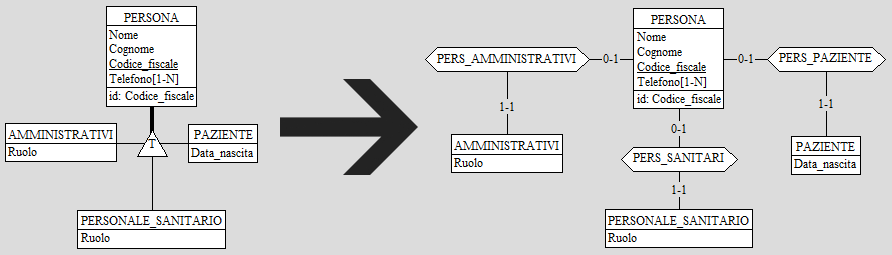
\includegraphics[width=\textwidth]{img/ger_persona_complete.png}
	\caption{Schema del collasso della gerarchia \emph{Persona}.}
	\label{img:ger_persona_complete}
\end{figure}

\subsection{Eliminazione di attributi multivalore}
L'unico attributo multivalore presente nello schema è \emph{Telefono} nell'entità \emph{Persona}. Non essendo nota a priori la cardinalità massima
si decide di trasformare l'attributo in un'entità \emph{Telefono} a parte associata a \emph{Persona} tramite la relazione \emph{Utenza}.

\subsection{Scelta degli identificatori principali}
Nello schema E/R sono già evidenziate tutte le chiavi primarie di tutte le entità, segue una breve spiegazione su alcuni identificatori non banali:

La sala è identificata dal numero ma anche dall'ospedale in cui si trovano, questo perché i numeri delle sale sono univoci solo all'interno della
struttura in cui si trovano e potrebbero esistere sale con lo stesso numero in strutture diverse.

Anche per le unità operative è stato scelto un identificatore composto dal nome dell'unità e dalla struttura in cui si trova, perché potrebbero esistere
unità operative con stesso nome in strutture diverse.

Essendo l'inventario proprio di ogni ospedale anche i codici di inventario dell'attrezzatura sono in relazione all'ospedale in cui si trovano.

L'identificativo dell'appuntamento è inoltre composto dalla sala in cui si svolge, dalla data, e dall'ora. Questo impedisce che ci siano 2 appuntamenti che
iniziano nello stesso luogo nello stesso momento, ma non la sovrapposizione sfalsata di 2 appuntamenti che quindi andrà gestita diversamente.

\end{document}